Los resultados se muestran de modo que las modifcaciones se van agregando para mejorar el desempeño del algoritmo. Primero se presenta el cambio en metaheurística seguido del cambio en la función de fitness posteriormente se considera la extensión de vecindad planteada y por último el cambio de representación. El orden es el siguiente:
\begin{enumerate}
    \item ILS con vecindad N7 y makespan como función de fitness.
    \item ILS con diferentes funciones de fitness.
    \item ILS con extensión de vecindad N7.
    \item ILS con la representación y vecindades propuestas.
\end{enumerate}
\section{ILS con vecindad N7}
Estos resultados sirven como una base para determinar si las modificaciones posteriores resultan en mejoras apreciables.

Se muestran los resultados de manera gráfica para facilitar su visualización. Los resultados detallados se encuentran en el apéndice \ref{app:resn7ils}. Para cada instancia se muestra la mediana del error relativo de los resultados con respecto a los mejores resultados reportados en la literatura mostrados en el apéndice \ref{tab:sota}. 

\begin{figure}[H]
    \begin{subfigure}{\textwidth}
        \centering
        %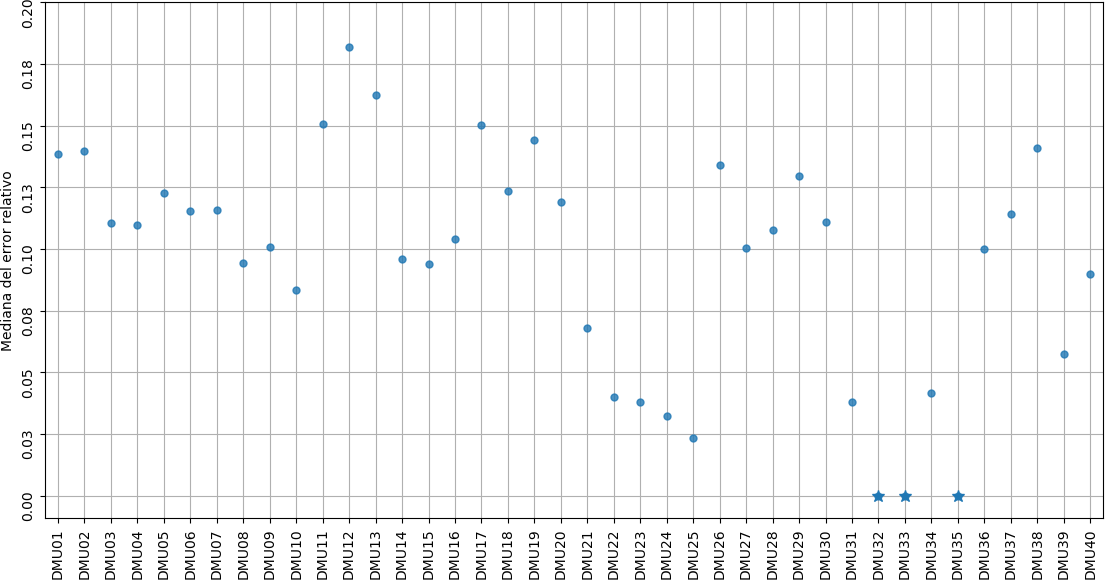
\includegraphics[height=.78\textwidth,width=.95\textheight,angle=270]{Imagenes/resn7ils1.png}
        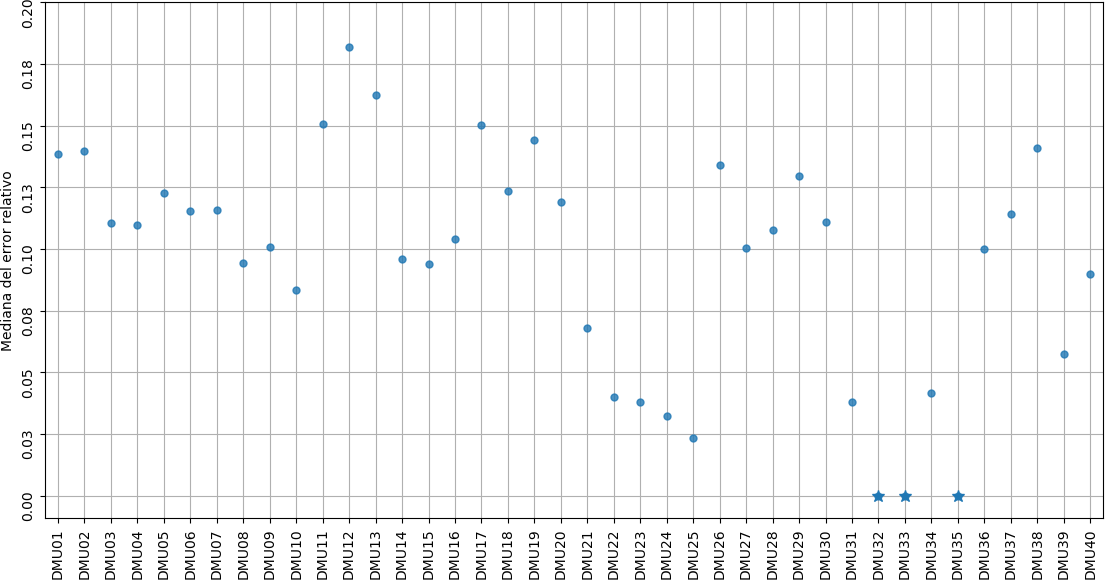
\includegraphics[scale=.65]{Imagenes/resn7ils1.png}
        \caption{Resultados para las instancias \textbf{DMU01-40}}
    \end{subfigure}
\end{figure}
\begin{figure}[H]\ContinuedFloat
    \begin{subfigure}{\textwidth}
        \centering
        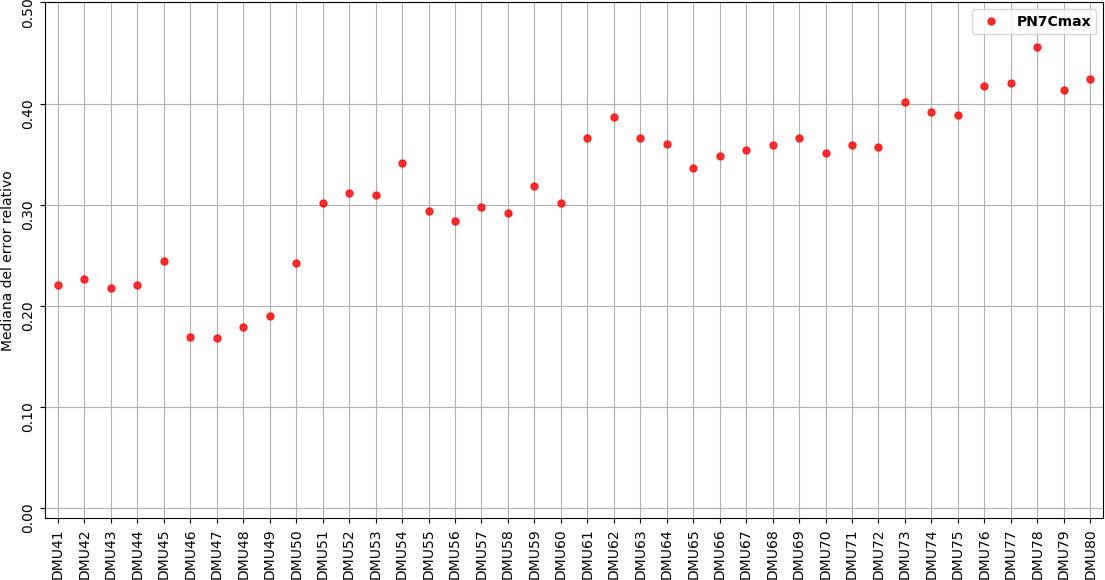
\includegraphics[scale=.65]{Imagenes/resn7ils2.png}
        \caption{Resultados para las instancias \textbf{DMU41-80}}
    \end{subfigure}
    \caption{Resultados para la propuesta más simple. Se marcan los casos en los que se llegó a la mejor solución conocida.}
\end{figure}

Podemos observar que la mediana del error relativo para la segunda mitad de las instancias es considerablemente mayor que para la primera mitad. Estos resultados sirven como un punto de comparación para todas modificaciones.

\section{Función de fitness}
  La función de fitness se obtiene al construir la dupla formada por el makespan y la característica en ese orden. Para determinar cuál es la que obtiene mejores resultados las modificaciones se comparan a pares en cada instancia. Si se encuentra que la diferencia entre dos modificaciones es estadísticamente significativa, se le suma un punto a la ganadora y se le resta uno a la perdedora.
Para determinar si los conjuntos de resultados muestran diferencias estadísticamente significativas se utiliza la prueba de Wilcoxon con un nivel de significancia de $0.01$. 

Los resultados para las propuestas mostradas en \ref{prop:fitness} pueden verse de manera condensada en la siguiente figura. El cuadro $(i,j)$ muestra el número de veces que $i$ fue mejor que $j$.\\
Todas las pruebas se realizaron con la vecindad N7. Se muestra también una tupla construida con las características que obtuvieron mejores resultados. Estas características se ordenan de acuerdo a su número de comparaciones ganadas totales.
\begin{figure}[H]
    \centering
    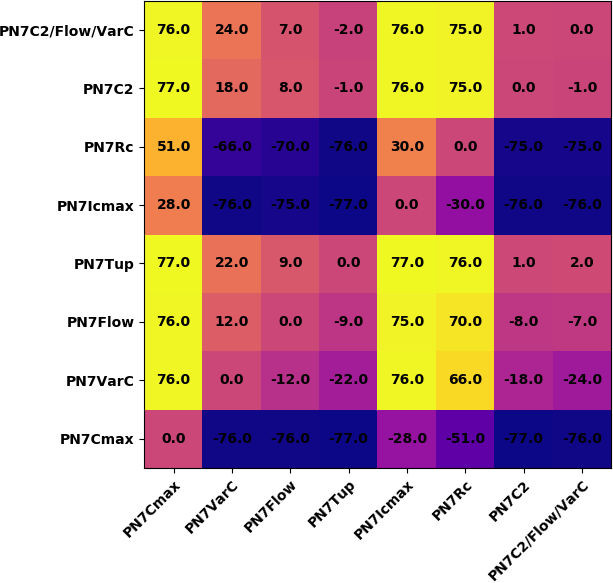
\includegraphics[scale=.8]{Imagenes/fitnesscomp.png}
    \caption{Condensado de los resultados para las modificaciones a la función de fitness. }
\end{figure}

Los mejores resultados se obtienen al construir la tupla mencionada previamente por lo que de ahora en adelante la función de fitness queda fija de esta manera y en los resultados subsecuentes solo se considera este caso. Los resultados detallados se muestran en el apéndice \ref{app:resn7tuple}.

\section{Extensión a vecindad N7}
Los resultados para la extensión que considera movimientos con espacios de inactividad de las máquinas se comparan con los mejores mostrados en la sección pasada. Se sigue el mismo procedimiento que en la sección anterior para hacer esta comparación.

\begin{figure}[H]
    \centering
    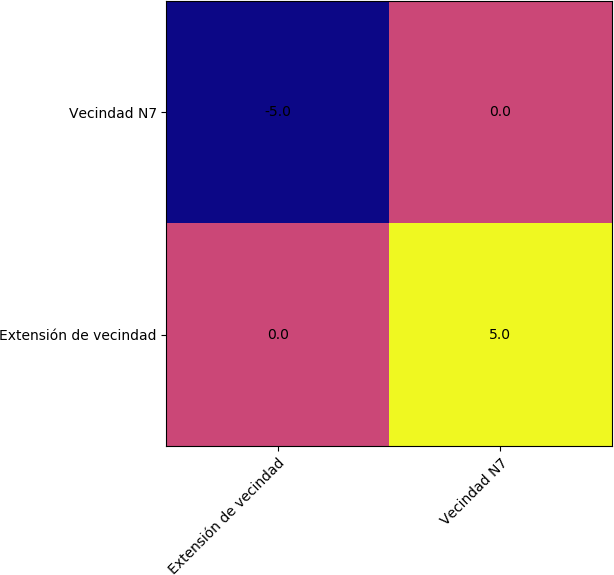
\includegraphics[scale=.7]{Imagenes/n8vsn7.png}
    \caption{Resultados de la comparación}
\end{figure}

También se muestra de manera gráfica los resultados para todas las instancias junto con los mejores resultados de la sección anterior. Los resultados detallados para la extensión propuesta se encuentran en el apéndice \ref{app:resn8tuple}.

\begin{figure}[H]
    \begin{subfigure}{\textwidth}
        \centering
        %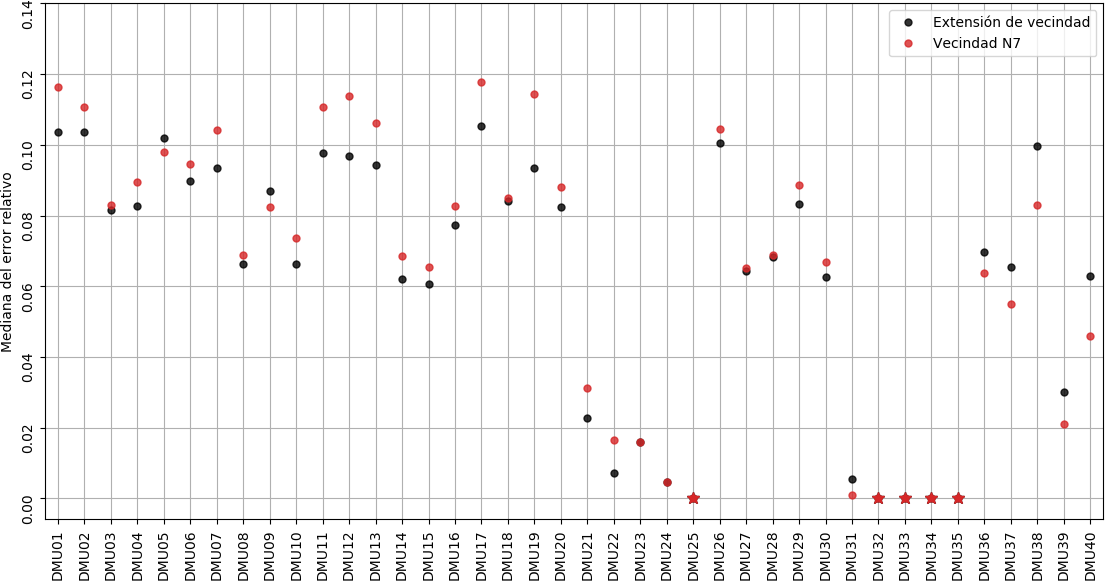
\includegraphics[height=.78\textwidth,width=.95\textheight,angle=270]{Imagenes/n8vsn7err1.png}
        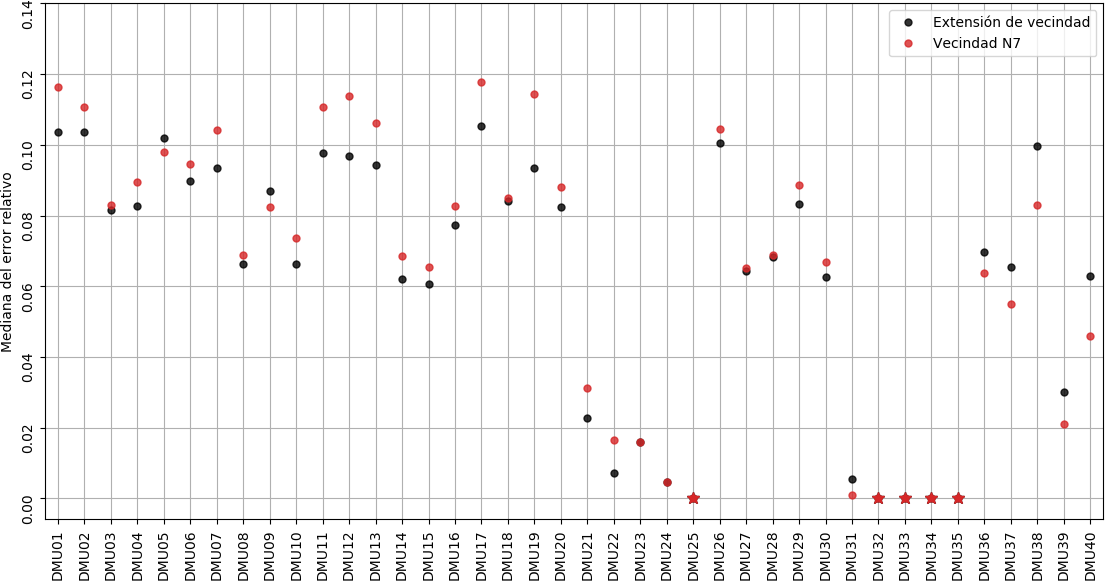
\includegraphics[scale=.6]{Imagenes/n8vsn7err1.png}
        \caption{Resultados para las instancias \textbf{DMU01-40}}
    \end{subfigure}
\end{figure}
\begin{figure}[H]\ContinuedFloat
    \begin{subfigure}{\textwidth}
        \centering
        %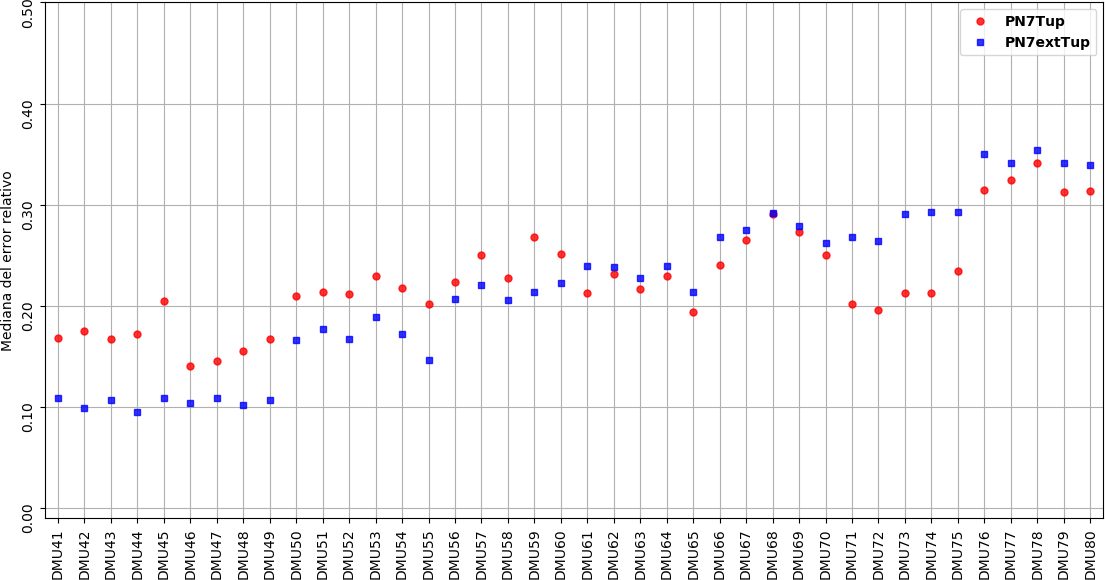
\includegraphics[height=.78\textwidth,width=.95\textheight,angle=270]{Imagenes/n8vsn7err2.png}
        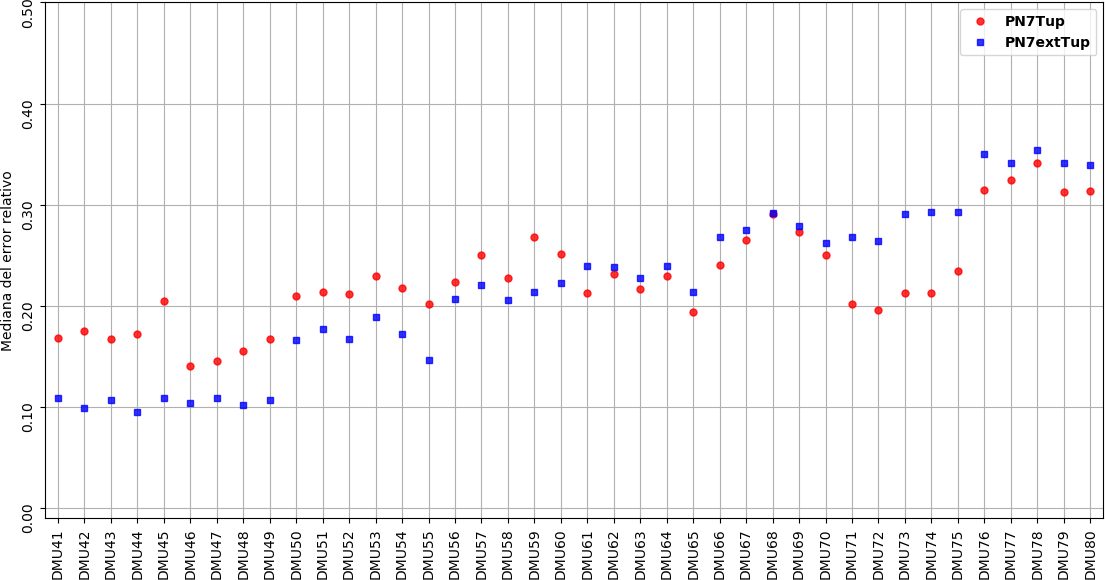
\includegraphics[scale=.6]{Imagenes/n8vsn7err2.png}
        \caption{Resultados para las instancias \textbf{DMU41-80}}
    \end{subfigure}
    \caption{Resultados para ambos métodos. Se marcan los casos en los que se llegó a la mejor solución conocida.}
\end{figure}

\section{Cambio de representación y vecindad}
El cambio de representación y vecindad se compara con las dos propuestas previas. Se sigue el mismo procedimiento mencionado para determinar si hay una diferencia significativa entre los resultados obtenidos.
\begin{figure}[H]
    \centering
    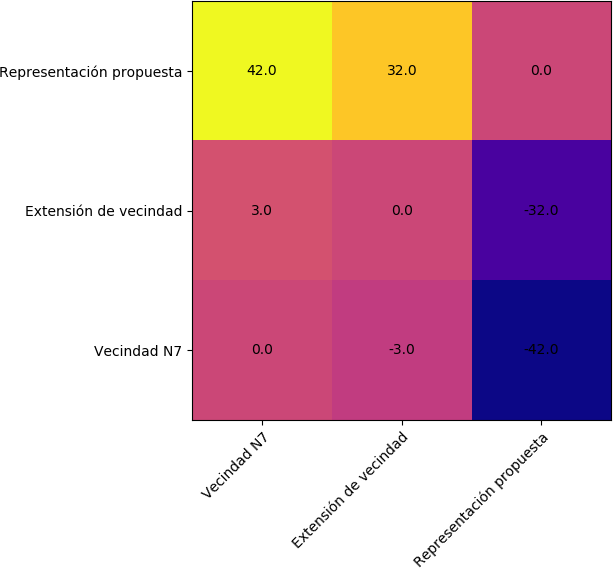
\includegraphics[scale=.7]{Imagenes/prn7n8comp.png}
    \caption{Resultados de la comparación entre los tres métodos.}
\end{figure}
También se muestra la mediana del error relativo alcanzado por los distintos métodos. Los resultados detallados para la extensión de vecindad se encuentran en el apéndice \ref{app:resprtuple}.

\begin{figure}[H]
    \begin{subfigure}{\textwidth}
        \centering
        %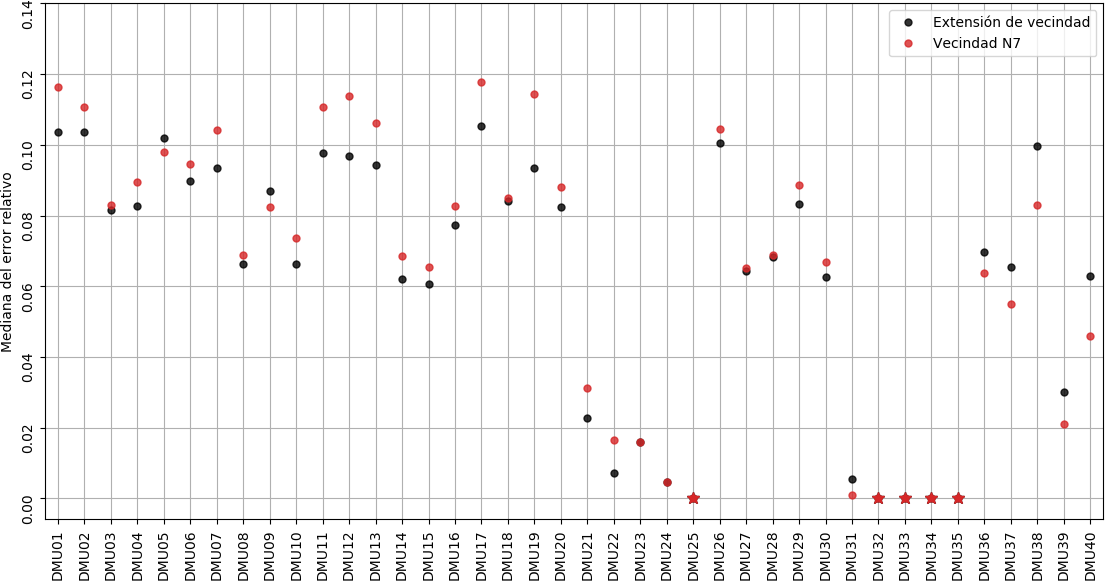
\includegraphics[height=.78\textwidth,width=.95\textheight,angle=270]{Imagenes/n8vsn7err1.png}
        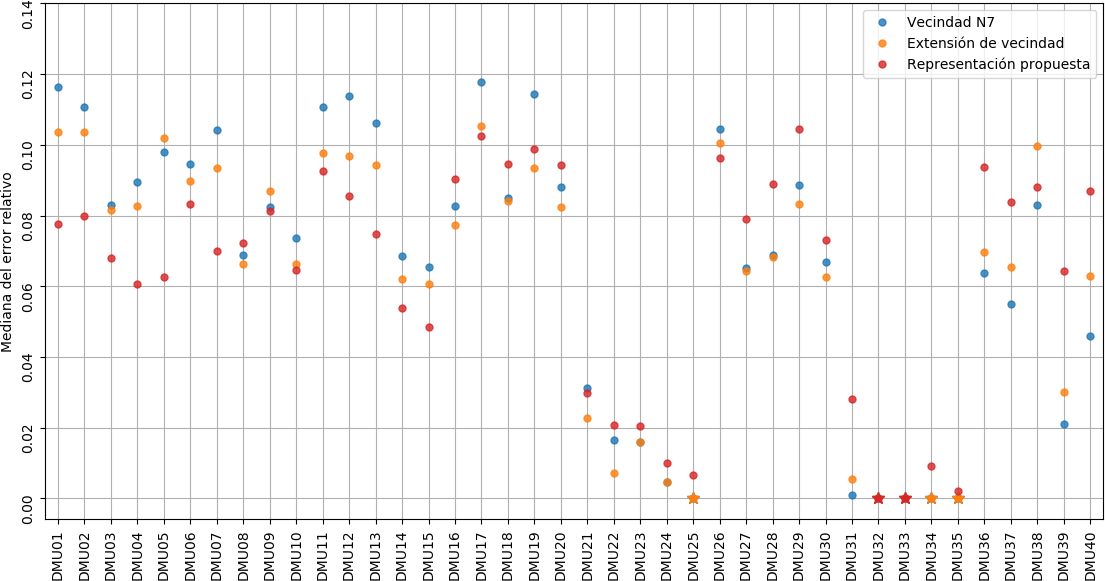
\includegraphics[scale=.6]{Imagenes/prvsn7vsn8err1.png}
        \caption{Resultados para las instancias \textbf{DMU01-40}}
    \end{subfigure}
\end{figure}
\begin{figure}[H]\ContinuedFloat
    \begin{subfigure}{\textwidth}
        \centering
        %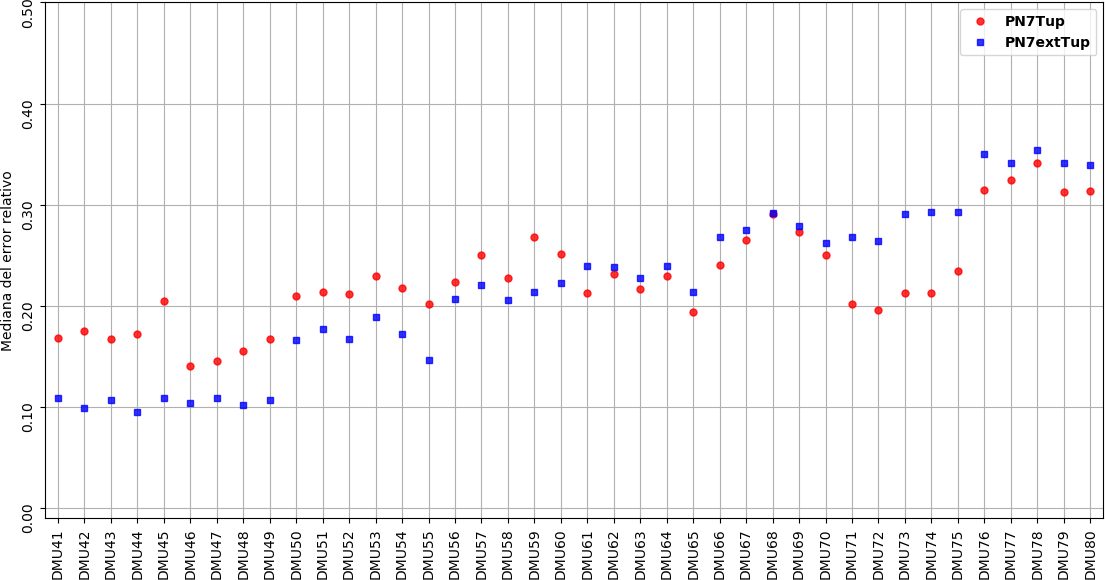
\includegraphics[height=.78\textwidth,width=.95\textheight,angle=270]{Imagenes/n8vsn7err2.png}
        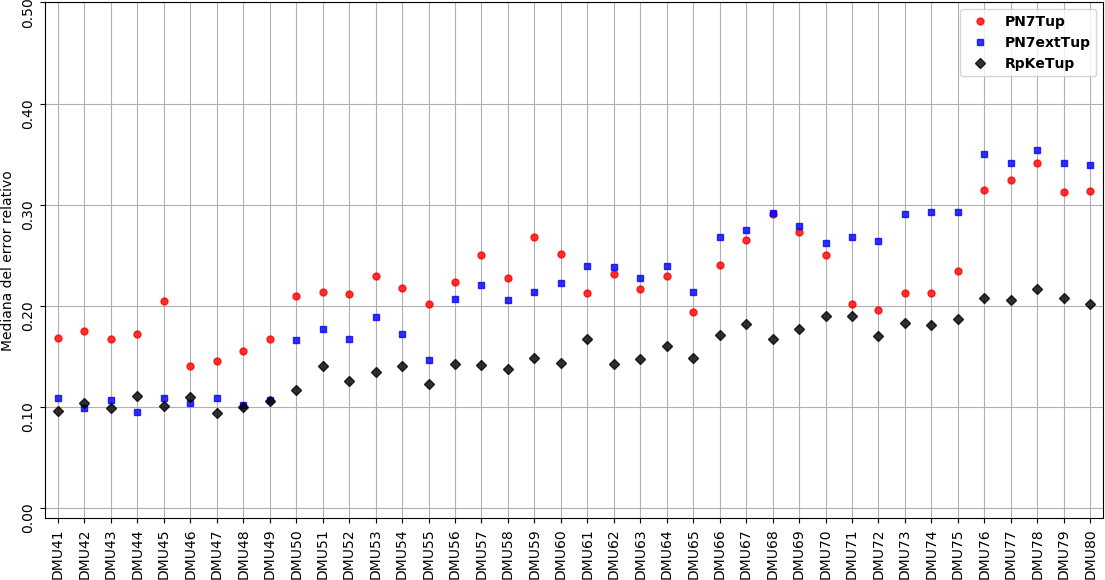
\includegraphics[scale=.6]{Imagenes/prvsn7vsn8err2.png}
        \caption{Resultados para las instancias \textbf{DMU41-80}}
    \end{subfigure}
    \caption{Resultados para ambos métodos. Se marcan los casos en los que se llegó a la mejor solución conocida.}
\end{figure}


Para resaltar las diferencias entre los dos métodos se tomó la instancia en la que se obtuvieron los resultados más dispares, en este caso fue la \textbf{DMU78} y se registró para cada óptimo local visitado su makespan así como el tamaño de su vecindad.

\begin{figure}[H]
    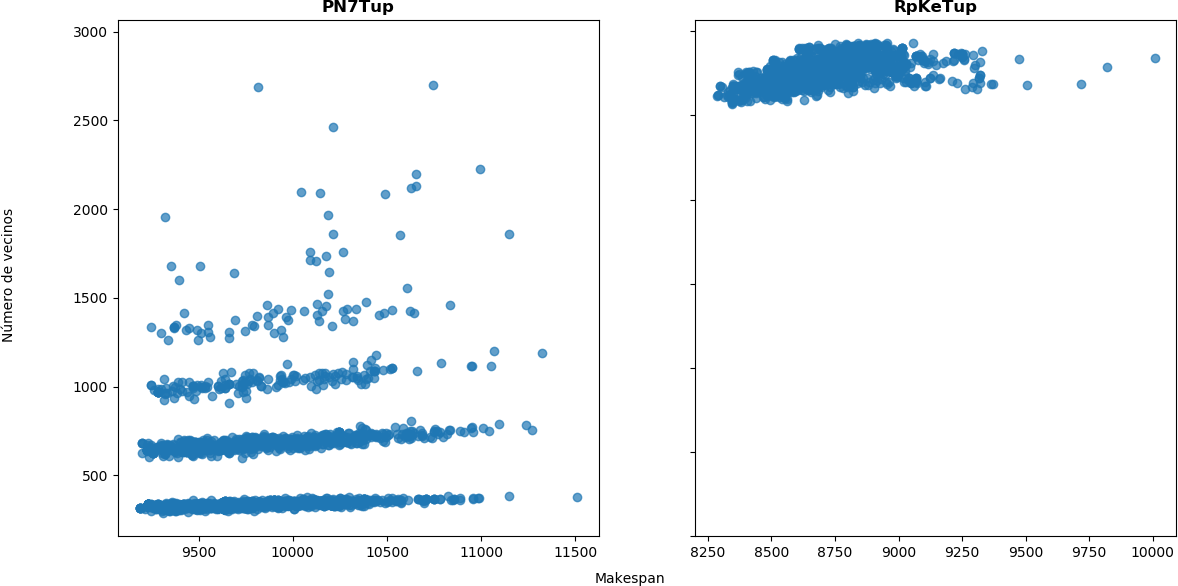
\includegraphics[scale=.6]{Imagenes/compvec78.png}
    \caption{Comparación de tamaño de la vecindad contra makespan de los óptimos locales para la instancia \textbf{DMU78} }
    \label{fig:mattgraph}
\end{figure}

Otro modo de visualizar las diferencias entre ambas representaciones también se presentan diagramas de caja para la diferencia relativa relativa del makespan de los óptimos locales con sus vecinos. Esto nos da una idea de cómo se relacionan las soluciones de acuerdo con su makespan. Si estos valores son muy cercanos entre sí esto nos da un indicio de la suavidad del paisaje de búsqueda.
\begin{figure}[H]
    \begin{subfigure}{\textwidth}
        \centering
        %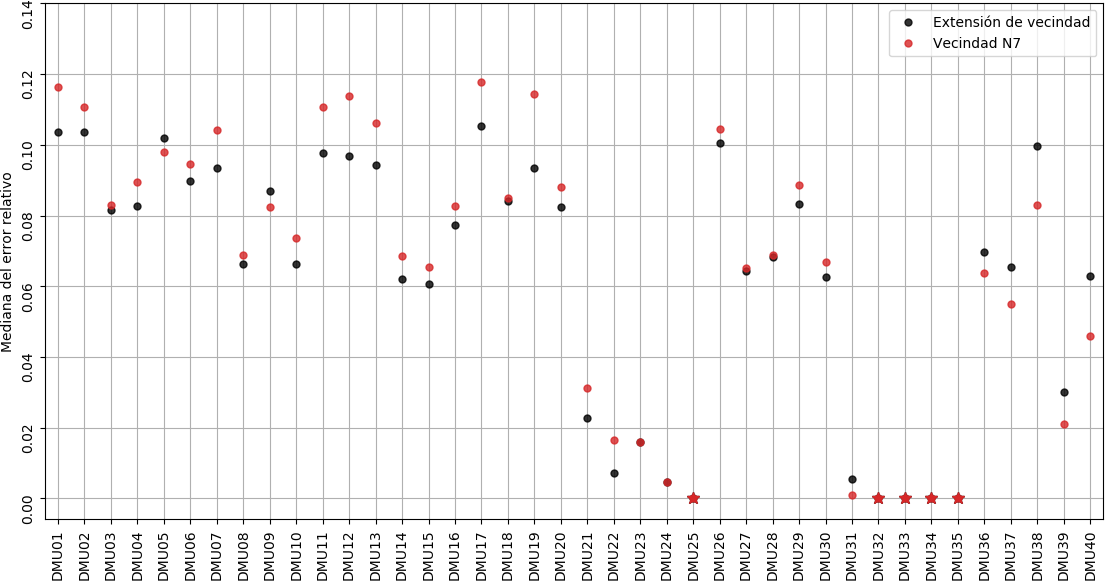
\includegraphics[height=.78\textwidth,width=.95\textheight,angle=270]{Imagenes/n8vsn7err1.png}
        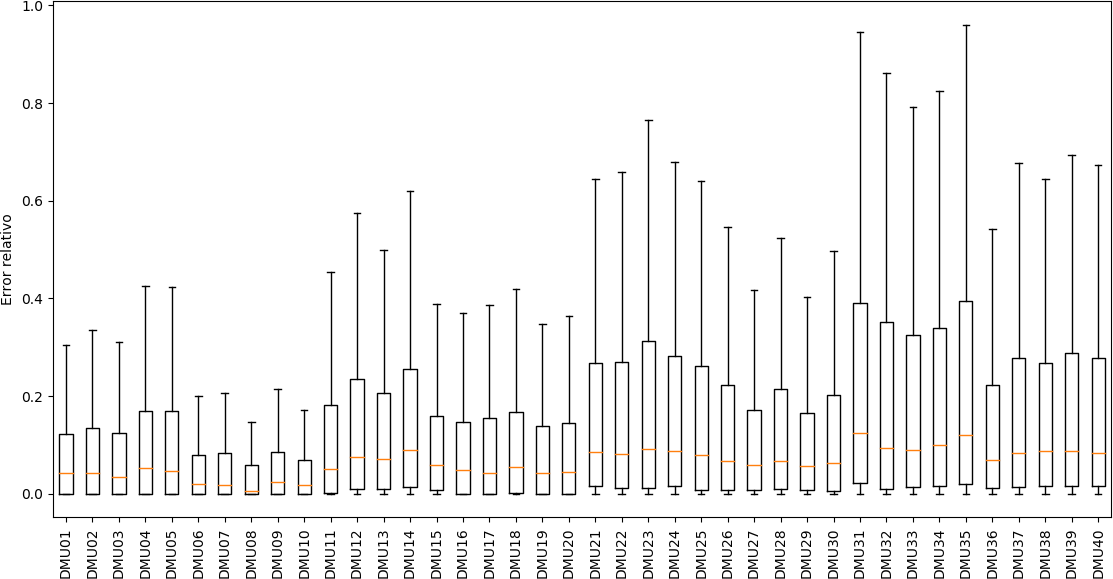
\includegraphics[scale=.6]{Imagenes/bxpn7_1.png}
        \caption{Representación original con vecindad n7 instancias \textbf{DMU01-40}}
    \end{subfigure}
\end{figure}
\begin{figure}[H]\ContinuedFloat
    \begin{subfigure}{\textwidth}
        \centering
        %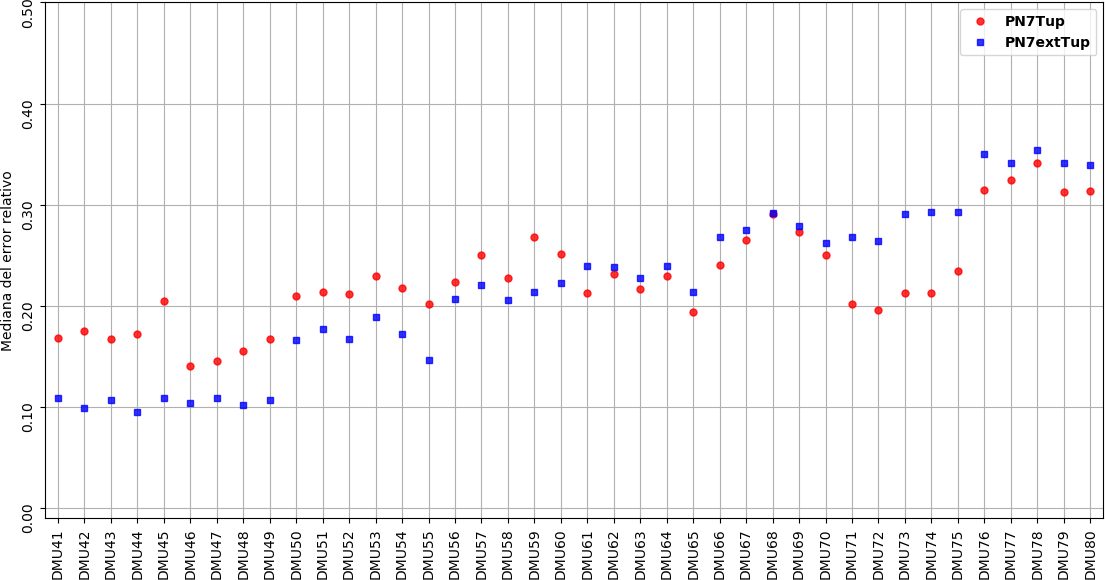
\includegraphics[height=.78\textwidth,width=.95\textheight,angle=270]{Imagenes/n8vsn7err2.png}
        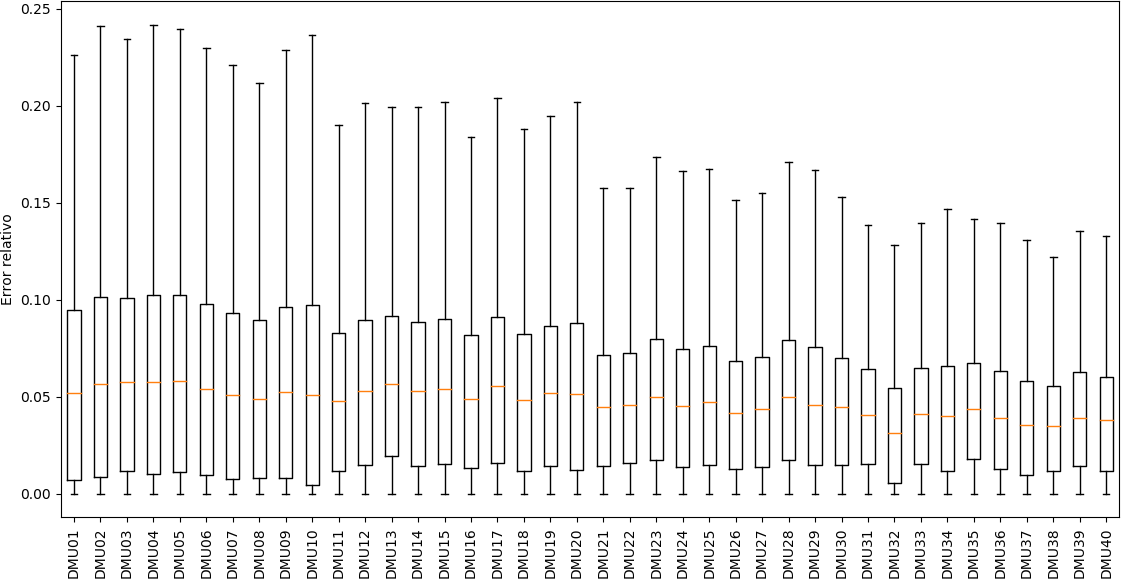
\includegraphics[scale=.6]{Imagenes/bxppr_1.png}
        \caption{Representación propuesta instancias \textbf{DMU01-40}}
    \end{subfigure}
    \caption{Diagramas de caja de la diferencia relativa en makespan de un óptimo local con sus vecinos}
    \label{fig:bxp1}
\end{figure}

\begin{figure}[H]
    \begin{subfigure}{\textwidth}
        \centering
        %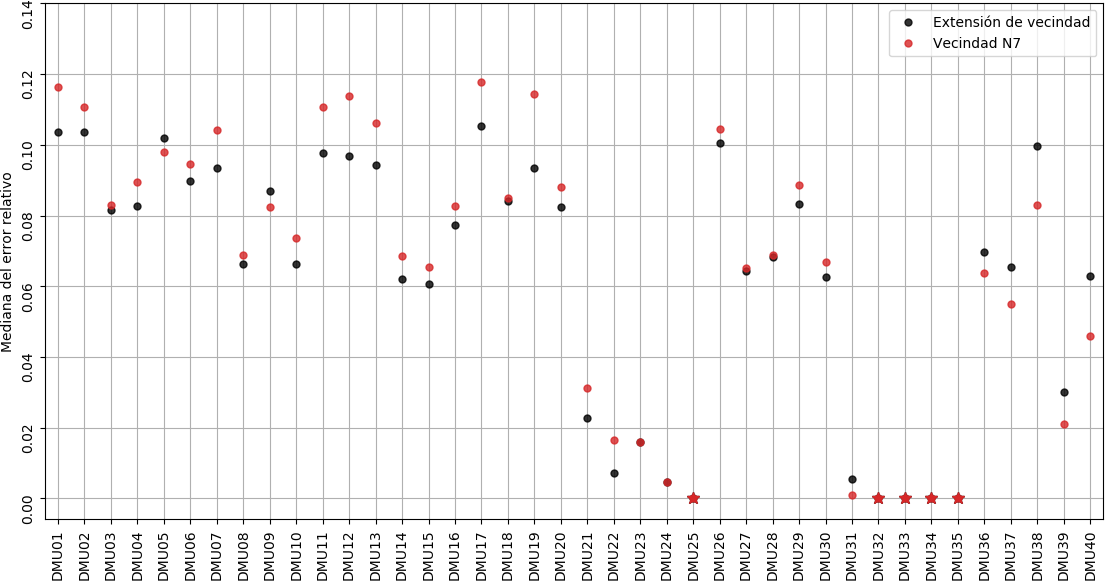
\includegraphics[height=.78\textwidth,width=.95\textheight,angle=270]{Imagenes/n8vsn7err1.png}
        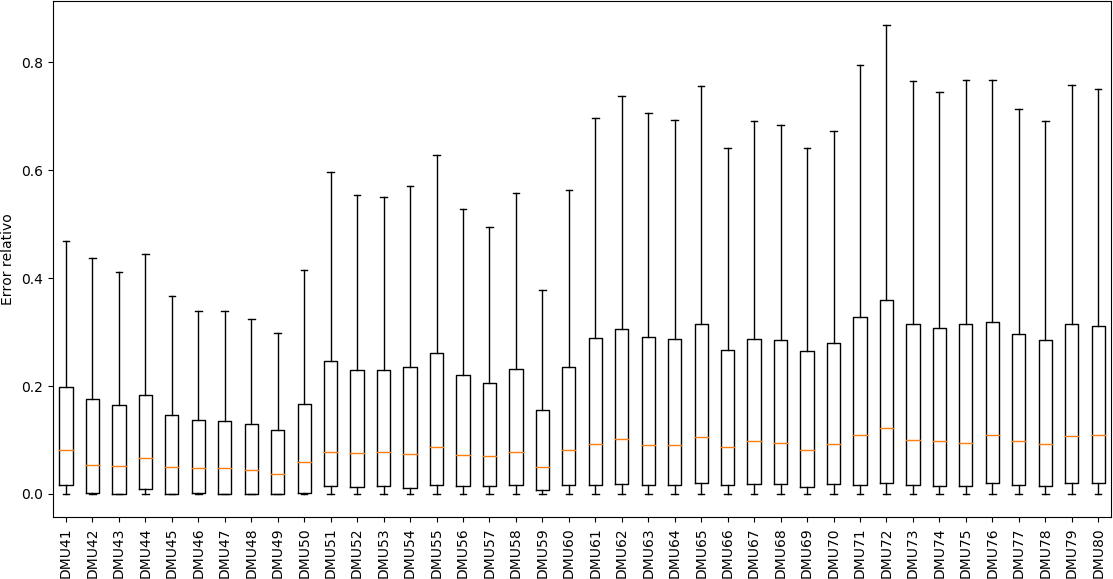
\includegraphics[scale=.6]{Imagenes/bxpn7_2.png}
        \caption{Representación original con vecindad n7 instancias \textbf{DMU41-80}}
    \end{subfigure}
\end{figure}
\begin{figure}[H]\ContinuedFloat
    \begin{subfigure}{\textwidth}
        \centering
        %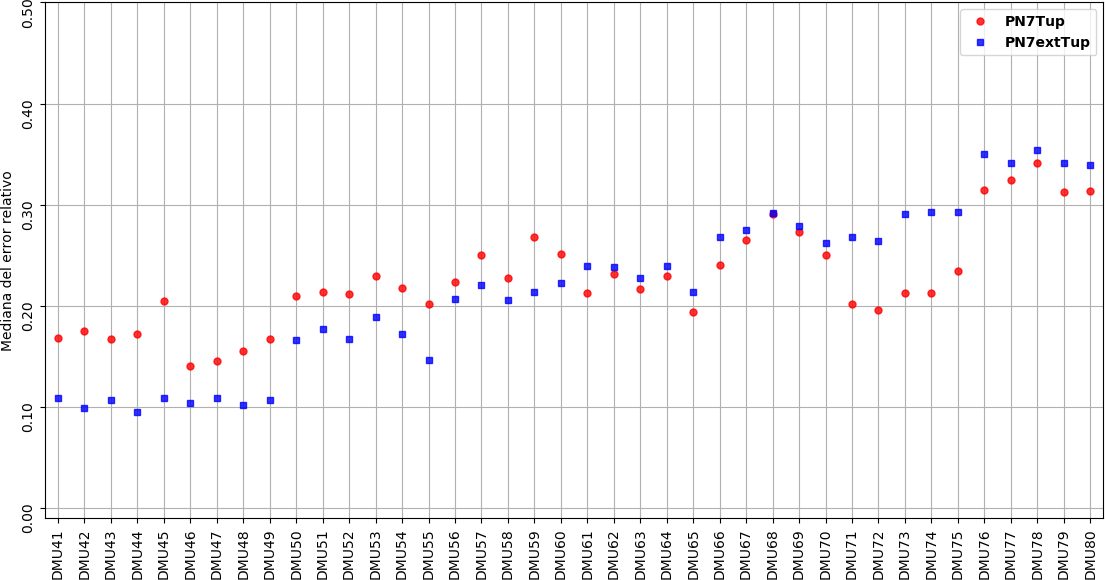
\includegraphics[height=.78\textwidth,width=.95\textheight,angle=270]{Imagenes/n8vsn7err2.png}
        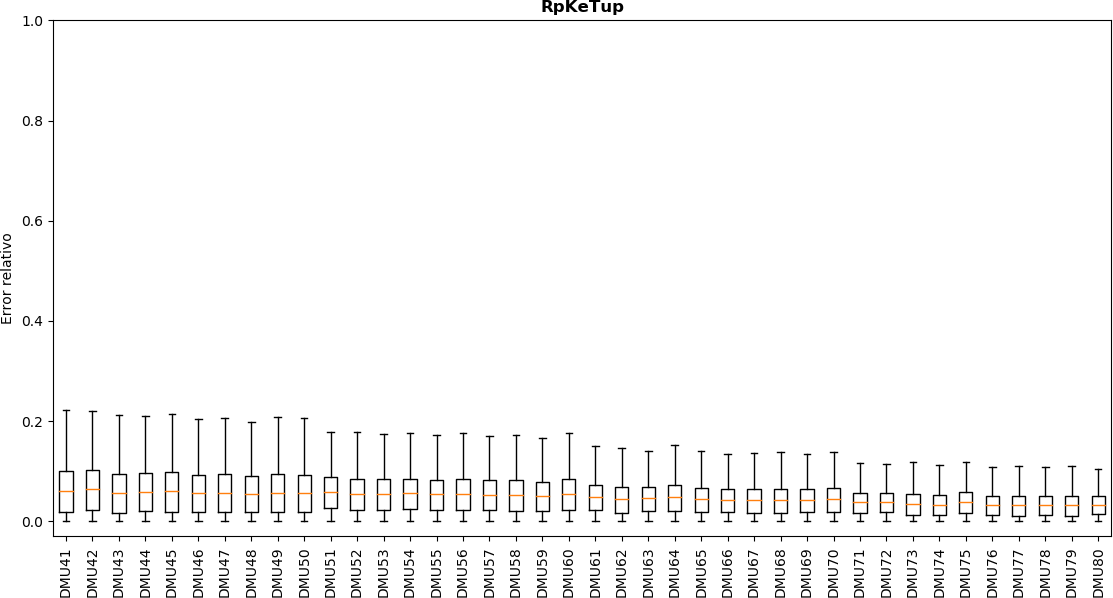
\includegraphics[scale=.6]{Imagenes/bxppr_2.png}
        \caption{Representación propuesta instancias \textbf{DMU41-80}}
    \end{subfigure}
    \caption{Diagramas de caja de la diferencia relativa en makespan de un óptimo local con sus vecinos}
    \label{fig:bxp2}
\end{figure}

En las figuras \ref{fig:bxp1} y \ref{fig:bxp2} observamos que los vecinos de los óptimos locales para la nueva representación y vecindad son más parecidos.
